
\documentclass{stat572Style}
\usepackage{natbib}
\usepackage{amssymb}
\usepackage{graphicx}
\usepackage{amsmath}
\usepackage{wrapfig}
\usepackage{url}
\usepackage{subfigure}
%%\setlength{\oddsidemargin}{0.25in}
%%\setlength{\textwidth}{6in}
%%\setlength{\topmargin}{0.5in}
%%\setlength{\textheight}{9in}

\renewcommand{\baselinestretch}{1.5} 

\bibliographystyle{plainnat}

\usepackage{color}
\usepackage{ulem}
\newcommand{\vmdel}[1]{\sout{#1}}
\newcommand{\vmadd}[1]{\textbf{\color{red}{#1}}}
\newcommand{\vmcomment}[1]{({\color{blue}{VM's comment:}} \textbf{\color{blue}{#1}})}
\newcommand{\hdcomment}[1]{({\color{red}{HD's comment:}} \textbf{\color{red}{#1}})}

\begin{document}
%%\maketitle

\begin{center}
  {\LARGE A Review of Lagrangian Time Series Models for Ocean Surface Drifter Trajectories (Sykulski et al. (2016))}\\\ \\
  {Hannah Director \\ 
    Department of Statistics, University of Washington Seattle, WA, 98195, USA
  }
\end{center}



\begin{abstract}
  This report reviews the spectral analysis method for modeling ocean surface drifters proposed by \citet{Sykulski2016}. 
  Previous methods to model drifters are discussed along with the authors' model. 
    Where relevant to understanding the model of \citet{Sykulski2016},  spectral analysis, Mat\'{e}rn covariances, the complex-valued Ornstein-Uhlenbeck process, and the Whittle likelihood are reviewed. 
     To conclude the report, we evaluate the strengths and weaknesses of this method. 
  \end{abstract}

\section{Introduction}
\citet{Sykulski2016} present a multi-component spectral model for analysis of data transmitted by ocean surface drifters. 
Drifters are free-floating  instruments that transmit their location at regular time intervals,  creating a \textbf{\it{Langrangian time series}}, or a sequence of spatial locations over time. 
Figure \ref{fig: fig1} shows a sample 250-day drifter trajectory. 
Oceanographers use these time series to increase understanding of  ocean circulation patterns.
Published in January 2016 in the \textbf{\it{Journal of the Royal Statistical Society Series C}}, this paper makes a notable contribution to the statistical literature by illustrating how to directly embed knowledge of a physical system into a stochastic model. 
 \begin{figure}[h!]
  \centering
    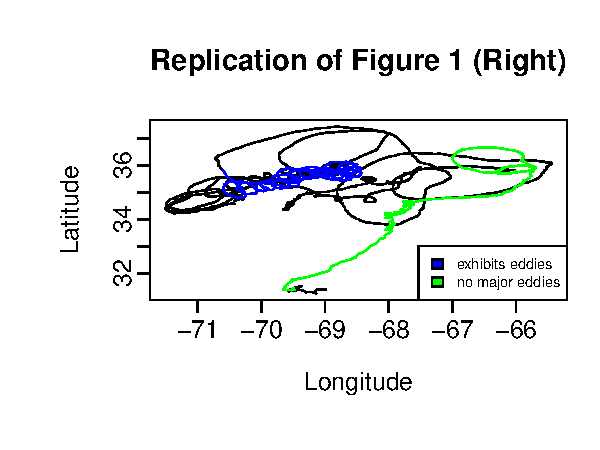
\includegraphics[width=.6\textwidth]{ReplicatedFigures/fig1.pdf}
        \caption{A 250-day sample drifter trajectory with two 50-day periods highlighted in green and blue. The time period highlighted in green is not affected by eddies while the time period highlighted in blue is.}
        	\label{fig: fig1}
\end{figure}
 
\par
The motion of parcels of water moving over changing latitudes is known to have a rotational component. 
Because the Earth has  different diameter at different latitudes, the speed of objects moving with Earth's rotation varies across latitudes.  
This induces a phenomena known as the Coriolis Effect, whereby very fast moving objects or objects observed over long periods, such as drifters, end up moving at speeds that are different than the Earth beneath them as they change latitude. 
Viewed from a stationary reference frame, this creates circular motions, or inertial oscillations. 
These motions have known frequencies, referred to as inertial frequencies, which take on positive values in the Southern hemisphere and negative values in the Northern hemisphere corresponding to the different directions objects rotate in the two hemispheres.
 Oceanographers  are interested in detecting deviations from these frequencies, as they are thought to indicate eddies, or persistent circular wave patterns \citep{Kunze1985}.
  However, the ocean has a constant turbulent background flow which makes identifying eddies in real data difficult \citep{ Elipot2010}.
 The majority of the previous work in oceanography has focused on detecting eddies using satellite altimetry rather than drifter data (see \citet{Isern2003} or \citet{Fu2010}, for example), so there is limited work on detecting eddies from drifters.
\citet{Shoosmith2005} and \citet{Lankhorst2006} do identify eddies by finding periods of repeated looping in the drifters' trajectories with a simple autoregressive model.
 Similarly, \citet{Boebel2003} calculate the curvature of the trajectory  and then classify eddies as periods of consistent rotations in one direction. 
 \citet{Sykulski2016} assert that they are the first to identify eddies by explicitly modeling inertial oscillations within a stochastic model.  
 \par
In achieving this result, several statistical advances are made.  
The authors introduce an additive spectral domain model that has components corresponding to both the turbulent background and the inertial oscillations. 
The Mat\'{e}rn covariance commonly used in spatial statistics \citep{Gneiting2012} is applied for the first time to model the turbulent background. 
Because of its flexibility, this covariance structure is shown to have more desirable features than previously-used stochastic models. 
Inertial oscillations are modeled with a complex-valued Ornstein-Uhlenbeck (OU) \citep{Arato1962, Jeffreys1968}, which provides a stochastic equivalent to an accepted set of coupled differential equations describing inertial oscillations. 
Further statistical innovation is employed in fitting the model with a variation on standard Whittle likelihood that compensates for both bias and aliasing and in allowing for non-stationarity through time-varying parameter estimates.
\par
The remainder of this report proceeds as follows.
 After a succinct review of spectral analysis, Section 2 discusses the model for the drifters and the methods used to fit it. 
 Section 3 presents the paper's results including analysis of a long time series with time-varying parameters and an application from a simulated model. 
We conclude the paper with a discussion of the value and limitations of the approach taken by \citet{Sykulski2016}. 






\section{Methods}
			

	\subsection{Spectral Analysis}
	\label{sec: specAnalysis}
	\indent We briefly review spectral analysis as all the analysis in \citet{Sykulski2016} is done in the spectral domain.   
	More thorough coverage of this material can be found in  \citet{Percival1993}, for example. 
	From a statistical perspective, a time series, $z(t)$, real or complex-valued,  can be understood as a realization of a stochastic process over time, where  $t = \{1,2,...,n\}$ index the observed time points.  
	Time series are often modeled as the sums of periodic functions, which, using Euler's formula, can be represented compactly as sums of appropriately-weighted complex exponentials. 
	Moreover, data in the time domain can easily be related to data in the frequency domain and vice versa using the Fourier or inverse Fourier transformations,
	\begin{align}
Z_{m} = \frac{1}{2T} \int_{-T}^{T}z(t)e^{-i\omega_{m}t} dt && z(t) = \sum_{m=-\infty}^{\infty}Z_{m}e^{i \omega_{m} t},
\end{align}
where $T$ indicates the period \citep{Percival1993}. 
To understand the distribution of frequencies, the \textbf{\it{power spectral density}},
\begin{equation}
S_{z}(\omega) = \underset{T \rightarrow \infty}{\lim} \mathbb{E} \left(\frac{1}{2T} \left| \int_{-T}^{T} z(t) e^{-i \omega t}dt \right|^{2} \right),
\end{equation}
is often employed. 
This quantity represents the variance (or power) associated with each frequency \citep{Percival1993}. 
Power spectral densities are useful for statistical modeling and can be related to the autocovariance sequence of a time series using  Fourier transformation.  
We define the autocovariance  for $z(t)$ as $s(\tau) = \mathbb{E}[z(t) z^{*}(t - \tau)] $ where $z^{*}(t)$ represents the complex conjugate of z(t). Letting $\tau$ be the time lag, we have
\begin{align}
\label{eq: fourierPair}
S_{z}(\omega) = \int_{-\infty}^{\infty}s_{z}(\tau) e^{-i\omega t}d \tau \Longleftrightarrow s_{z}(\tau) = \frac{1}{2\pi} \int_{-\infty}^{\infty}S_{z}(\omega) e^{i \omega t} d\omega 
\end{align}

\noindent \citep{Percival1993}. For an observed time series, the power spectral density is often estimated with the periodogram, where 
\begin{equation}
\label{eq: perio}
\hat{S}_{z}(\omega) = \frac{\Delta}{N} \left( \sum_{t=1}^{N} z(t) e^{-i \omega t \Delta} \right)^{2}
\end{equation}
\citep{Sykulski2013}. 
Although intuitively appealing, this estimator has known problems that stem from  sampling a time series at discrete intervals. 
Specifically, \textbf{\it{Aliasing}} refers to the fact that frequencies above the highest observable frequency cannot be captured, and, are instead, confounded with other frequencies in the spectrum.  
\textbf{\it{Leakage}} describes how as a result of convolution, power from one part of the spectral density function can be transferred to another part of the density. 


\subsection{Stochastic Model}
 To model a drifter's movement over time, the eastward and northward components of the drifter's velocity, denoted $u(t)$ and $v(t)$ respectively, are converted to a complex-valued velocity, $z(t) = u(t) + iv(t)$. 
 Separate stochastic models are introduced for the inertial oscillation and turbulent background components of the drifter's behavior. 
 Working in the frequency domain, the two components of the model are added together, creating a six-parameter spectral model. 
 Parameter estimates for this model are obtained via maximizing the model's blurred Whittle likelihood, a relatively new approximation to the true Whittle likelihood that compensates for bias and handles aliasing \citep{Sykulski2013}. 
 
\subsubsection{Inertial oscillations}
We begin by discussing the model for the inertial oscillations. 
In a deterministic setting, inertial oscillations are often modeled with the following set of coupled differential equations
\begin{align}
\label{eq: deterOsc}
\frac{\partial u }{\partial t}  + f_{0} \nu &= F - cu,\\ \nonumber
\frac{\partial v}{\partial t} - f_{0}u &= G - cv,
\end{align}
where $u$ and $v$ again represent eastward and northward velocities, $f_{0}$ represents the inertial frequency in radians per unit time, and $F$ and $G$ are forces related to the wind  \citep{Pollard1970}. 
Suppressing the dependence on $t$ and using the complex representation of the velocity,  we show that these relationships can be equivalently expressed as follows
\begin{align}
\label{eq:diffEqDeriv}
\nonumber
\frac{dz}{dt} &= \frac{\partial u}{dt} + i\frac{\partial v(t)}{dt} \\ \nonumber
dz &= (F - c u- f_{0}v)dt + i(G - cv + f_{0}u)dt\\ \nonumber
&= f_{0}(-v + iu)dt - c(u + iv)dt + (F + iG)dt\\ \nonumber
&= if_{0}(u + iv)dt - c(u + iv)dt + (F + iG)dt\\ 
&= (if_{0} - c)z dt + (F + iG)dt. 
\end{align}
\citet{Sykulski2016} further replace the wind forcing term, $(F + iG)dt$  with complex-valued Brownian increments \citep{Mandelbrot1968} to obtain a stochastic analogue for Equation \ref{eq:diffEqDeriv},
 \begin{equation}
\label{eq: ouEq}
dz(t) = (i f_{0} -c) z(t) dt + A d Q(t). 
\end{equation}  
Equation \ref{eq: ouEq}  is known as the complex-valued Ornstein-Uhlenbeck (OU) stochastic differential equation. 
In general,  OU processes are considered continuous-time equivalents to the AR(1) process. Specifically,  the univariate OU process is the only mean-zero, stationary, Gaussian, continuous Markov process, and, similarly the multivariate OU process is the only mean-zero $K$-variate process that is stationary, continuous, Gaussian, and Markov \citep{Schach1971}.
 The complex-valued OU process is the complex representation of a bivariate OU process.  
 In the formulation of Equation \ref{eq: ouEq}, $c > 0$ is a dampening parameter that forces the process to always eventually return to its mean position, $z = 0$.  
 The final term of Equation \ref{eq: ouEq} is a positive constant, $A$, multiplied by $dQ(t)$.  The term $Q(t), t \geq 0$ is a standard complex Wiener process,  meaning $Q(t) = Q_{1}(t) + i Q_{2}(t)$, where $Q_{1}(t)$ and $Q_{2}(t)$ are standard Wiener processes.
 We remind the reader that Wiener processes are the stochastic models originally used to represent Brownian motion. 
  Such a process $\{Q(t, \omega): t \geq 0\}$ on the measure space $(\omega, Q, P)$ must satisfy
\begin{enumerate}
\item $Q(0, \omega) = 0$ almost everywhere
\item $\{Q(t, \omega): t \geq 0\}$ is distributed normally on $(\Omega,Q, P)$
\item $Q(t + \tau, \omega) - Q(t, \omega)$ has mean 0 and variance $\tau$ for all $t, \tau > 0$
\end{enumerate}
\citep{Hida1980}. 

To identify and estimate shifts in the angular frequency, presumably caused by eddies, \citet{Sykulski2016} propose replacing the known inertial requency, $f_{0}$,  in Equation�~\ref{eq: ouEq} with  a free parameter, $\omega_{0}$, to be estimated by the data. 
If the estimated angular frequency differs from the inertial frequency, the angular frequency of the eddy can be calculated as $\omega_{eddy} = f_{0} - \omega_{0}$, since $\omega_{0}$ is a sum of the inertial and eddy frequencies.

For time series modeling, we are interested in the autocovariance of this process at different time lags. To derive the autocovariance as given in Equation 4 of \citet{Sykulski2016}, we follow \citet{Arato1999} and consider the bivariate rather than complex-valued OU process.
This is possible since the autocovariance of a complex-valued random variable $z(t) = u(t) + i v(t)$ with time lag $\tau >0$ is defined as 
\begin{equation}
\label{eq: expec}
s(\tau) = \mathbb{E}[z(t) z^{*}(t + \tau)] = \mathbb{E}[u(t)u(t + \tau)] + \mathbb{E}[(v(t) v(t + \tau)] + i(\mathbb{E}[u(t) v(t + \tau)] -\mathbb{E}[u(t + \tau)v( t)])
\end{equation}
 \citep{DeIaco2003}. The differential equations for components $u(t)$ and $v(t)$ can be expressed in matrix form as 
\begin{align}
\left( \begin{array}{c} du(t) \\ dv(t) \end{array} \right) &= 
\left( \begin{array}{cc} -c & -\omega_{0} \\ \omega_{0} & -c \end{array} \right) \left( \begin{array}{cc} u(t) \\ v(t) \end{array} \right) + \left( \begin{array}{c} A d Q_{1}(t) \\ Ad Q_{2}(t) \end{array} \right). 
\end{align}
For a bivariate OU process, the covariance matrix at time lag $\tau > 0$ is 
\begin{align}
\label{eq: bivOU}
\boldsymbol{C}(\tau) = \left( \begin{array}{cc} \mathbb{E}[u(t + \tau)u(t)] & \mathbb{E}[u(t + \tau)v(t)] \\ 
\mathbb{E}[v(t + \tau)u(t)] & \mathbb{E}[v(t + \tau) v(t)] \end{array} \right) = \exp \left\{ \left( \begin{array}{cc} -c & -\omega_{0} \\ \omega_{0} & -c \end{array} \right)\tau \right\}\boldsymbol{C}(0)
\end{align}
where $\boldsymbol{C}(0)$ gives the covariance matrix at the initial time, $t$ \citep{Schach1971}.  \citet{Sykulski2016} specify that at the initial time, $z(t) \sim$ N(0, $A^{2}/2c$). We also note $u(t)$ and $v(t)$ are uncorrelated at the initial time, giving $\mathbb{E}[u(t)v(t)] = \mathbb{E}[v(t) u(t)] = 0$. Thus, Equation \ref{eq: expec} simplifies to
\begin{equation}
\label{eq: s0}
s(0) = \frac{A^{2}}{2c} =  \mathbb{E}[u(t)^{2}] + \mathbb{E}[(v(t)^{2}]. 
\end{equation}
Since $u(t)$ and $v(t)$ are assumed to be the same type of process, Equation \ref{eq: s0} implies $\mathbb{E}[u(t)^{2}] =\mathbb{E}[(v(t)^{2}] = A^{2}/4c$, which means Equation \ref{eq: bivOU} can be expressed as 
\begin{align}
\label{eq: covDeriv}
 \boldsymbol{C}(\tau) =  \exp \left\{ \left( \begin{array}{cc} -c & -\omega_{0} \\ \omega_{0} & -c \end{array} \right)\tau \right\} \left( \begin{array}{cc} A^{2}/4c & 0 \\ 0 & A^{2}/4c \end{array} \right)  &= 
\frac{A^{2}}{4c} \exp (-c \tau) \left( \begin{array}{cc} \cos \tau \omega_{0} & - \sin \tau \omega_{0} \\ \sin \tau \omega_{0} & \cos \tau \omega_{0}  \end{array} \right) 
\end{align}
where the second equality can be seen by expanding the infinite series representations for $\exp(-c \tau)$, $\sin(\tau \omega_{0})$, and $\cos( \tau \omega_{0})$. 
Finally, using the values obtained in Equation \ref{eq: covDeriv} in Equation \ref{eq: expec}, we obtain the autocovariance  as defined in \citet{Sykulski2016}
\begin{align}
\label{eq: ouAC} \nonumber
s^{(o)}(\tau) & = \frac{A^{2}}{4c} \exp(-c\tau) 2(\cos \tau \omega_{0} + \sin \tau \omega_{0}) \\
&= \frac{A^{2}}{2c} \exp(i \omega_{0}\tau) \exp(-c|\tau|).
\end{align}
 The $(o)$ superscript denotes that this equation is for the OU component of the full model. Using Equation \ref{eq: fourierPair}, the corresponding power spectral density can be found to be\begin{align}
\label{eq:ouPSD}
S^{(o)}(\omega) &=  \int_{-\infty}^{\infty} s^{(0)}(\tau) \exp (-i \omega \tau) d \tau = \frac{A^{2}}{(\omega - \omega_{0}) + c^{2}}. 
\end{align}



\subsubsection{Turbulent Background}
The drifters' time series are also marked by the ocean's large-scale turbulence. 
The physics of ocean turbulence is summarized by \citet{Rhines1979}. 
Many models for ocean turbulence have been proposed, including several stochastic models \citep{Lacasce2008}. 
Within the oceanography literature, the stochastic models are designated  first-order \citep{Griffa1995, Falco2000}, second-order \citep{Sawford1991}, and third-order corresponding to  whether the velocity, acceleration, or hyperacceleration is modeled with a Markov process. 
However, calculation of the spectral slopes in observed data indicate that this class of models, referred to as \textbf{\it{integer order}},  does not always adequately reflect the ocean's behavior \citep{Rupolo1996, Sanderson1991}. Rather, \textbf{\it{fractional power models}}, such as fractional Brownian motion (FBM), would better reflect the observed behavior in some cases. 

Towards this end, the authors propose using a Mat\'{e}rn covariance structure \citep{Gneiting2012} for the turbulent background. 
The Mat\'{e}rn model has gained prominence in the spatial statistics literature due to its flexibility.
 In this context, the Mat\'{e}rn model proves useful, since it allows for both integer and fractional powers. 
 The Mat\'{e}rn model is defined either by its autocovariance 
\begin{align}
\label{eq:maternAC}
s^{(m)}(\tau) = \frac{B^{2}}{2^{\alpha - 1/2}\pi^{1/2} \Gamma(\alpha) h^{2 \alpha - 1}}(h|\tau|)^{\alpha - 1}\mathcal{K}_{\alpha - 1/2}(h|\tau|),
\end{align}
or power spectral density,
\begin{align}
\label{eq:maternPSD}
S^{(m)}(\omega) = \frac{B^{2}}{(\omega^{2} + h^{2})^{\alpha}},
\end{align}
where $\tau$ again denotes the time lag, $\Gamma(\alpha)$ is the gamma function,  $\mathcal{K}_{\eta}$ is a modified Bessel function of the second kind of order $\eta$ \citep{Stein2012}.  The superscript $(m)$ indicates that this is the Mat\'{e}rn part of the full model. 
The parameters to be estimated are the amplitude, $B$, the dampening, $h > 0$, and a smoothness parameter $\alpha > 1/2$.
 The parameter $\alpha$ is of particular importance, since it controls the smoothness, or degree of differentiability, of the process \citep{Fuentes2010}. 

The authors emphasize that the turbulent background models previously proposed are special cases of the Mat\'{e}rn model. 
This means that these models can still be obtained under the current model if model fitting leads to their parameter estimate values. 
They also highlight that that Mat\'{e}rn model is more appropriate than the other obvious choice of a fractional power model, FBM, since FBM does not have a bound on the velocities and tends to drift quite far from its mean.
 Figure \ref{fig: fmbMat} illustrates these differences by comparing the paths of a simulated particle obtained with a Mat\'{e}rn  covariance versus a FBM covariance. 

\begin{figure}[h!]
  \centering
    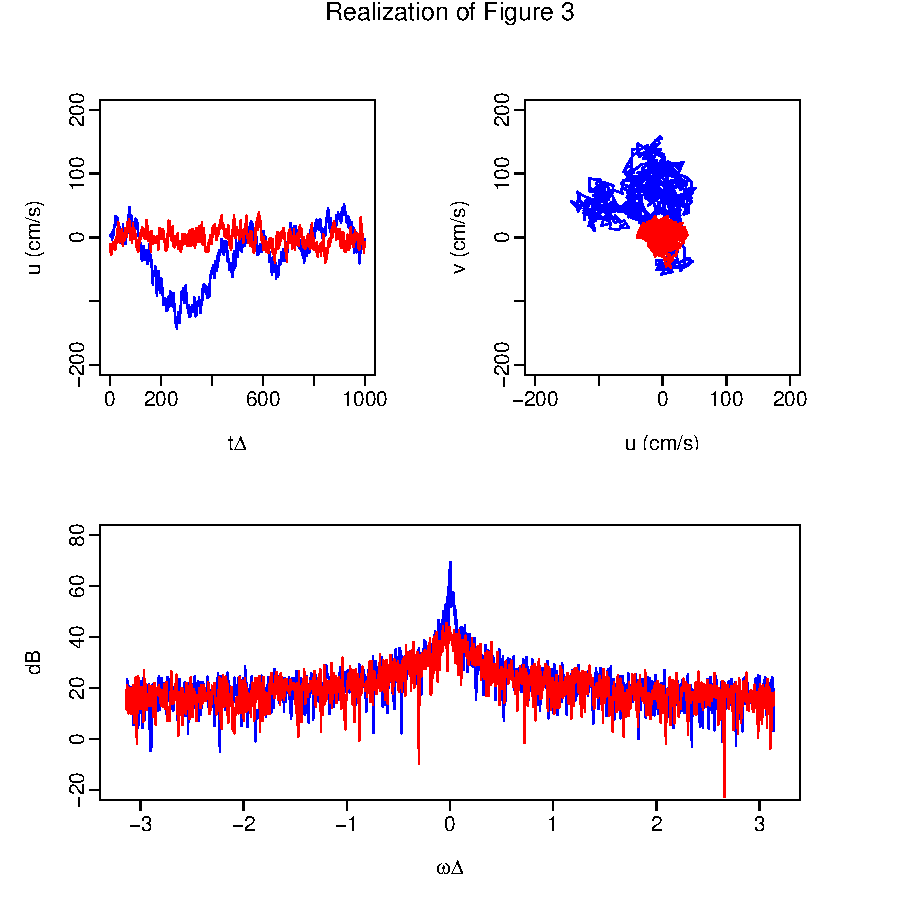
\includegraphics[width=.9\textwidth]{ReplicatedFigures/fig3.pdf}
        \caption{Simulated velocities obtained using FBM (blue) and Mat\'{e}rn (red)  processes. Top Left: The eastward component of the velocities. Top Right: The eastward and northward components of the velocities. Bottom: Periodograms of both processes on the decibel scale.}
        	\label{fig: fmbMat}
\end{figure}

\subsubsection{Overall Model}
Combining the inertial oscillation and turbulent background parts of the model is straightforward.
 To find both the autocovariance and power spectral densities, we can simply add the corresponding components of the inertial oscillation and turbulent background autocovariances. 
 Using Equations \ref{eq: ouAC} and \ref{eq:maternAC} and Equations \ref{eq:ouPSD} and \ref{eq:maternPSD}, we obtain
\begin{align}
\label{eq: fullSpec}
s(\tau ;\boldsymbol{\theta}) &= \frac{A^{2}}{2c} \exp(i \omega_{0}\tau) \exp(-c|\tau|) +  \frac{B^{2}}{2^{\alpha - 1/2}\pi^{1/2} \Gamma(\alpha) h^{2 \alpha - 1}}(h|\tau|)^{\alpha - 1}\mathcal{K}_{\alpha - 1/2}(h|\tau|)
,\\
S(\omega; \boldsymbol{\theta}) &= \frac{A^{2}}{(\omega - \omega_{0}) + c^{2}} + \frac{B^{2}}{(\omega^{2} + h^{2})^{\alpha}}.
\end{align}



\subsection{Fitting the Model}
\subsubsection{Blurred Whittle likelihood}
\par A recent technique introduced by \citet{Sykulski2013}  is used to fit the model.
 Referred to as \textbf{\it{blurred Whittle likelihood}}, this new likelihood builds on the well-known Whittle likelihood, a frequency-based approximation  to the time-domain likelihood that reduces computational cost. 
  Whittle likelihood is designed to approximate the likelihood for a univariate Gaussian process, $\boldsymbol{Z}$,  in the time domain that has the likelihood
\begin{align*}
l_{t}(\boldsymbol{\theta}) = - \frac{1}{2} \log \left|\boldsymbol{\Sigma}_{z}(\boldsymbol{\theta}) \right| - \frac{1}{2} Z^{T} \boldsymbol{\Sigma}_{z}^{-1}(\boldsymbol{\theta})\boldsymbol{Z},
\end{align*}
where $\boldsymbol{\theta}$ are the model parameters for a particular choice of covariance structure, $\boldsymbol{\Sigma}_{z}$,  and $t$ denotes the time domain  \citep{Sykulski2013}. 

 It is known that  the periodogram satisfies
\begin{equation}
\hat{S}_{z}(\omega) \overset{d}{\rightarrow} S(\omega) \chi^{2}_{2}/2
\end{equation}
under certain regularity conditions \citep{Contreras2006}. 
\citet{Whittle1953} combined this result with Fourier approximations to the true covariance structure and features of Toeplitz matrices to obtain the approximate likelihood
\begin{align}
\label{eq: bwl}
l_{\omega}(\boldsymbol{\theta}) 
&= -\sum_{\omega \in \Omega} \left[ \frac{\hat{S}_{z}(\omega)}{S(\omega;\boldsymbol{\theta})}  + \log  \{ S(\omega; \boldsymbol{\theta}) \}\right],
\end{align}
where the subscript $w$ indicates that this is a Whittle likelihood. 
Leveraging the fast Fourier transform \citep{Cooley1965}, this  likelihood can be evaluated in $\mathcal{O}(N log(N))$, where $N$ is the length of the time series. 
This is a notable increase in speed compared to the $\mathcal{O}(N^{3})$  required for time-domain likelihood  \citep{Sykulski2016}. 
  Nevertheless, this likelihood relies on the periodogram and so is affected by aliasing and leakage as discussed in Section \ref{sec: specAnalysis}. 
 
To improve on these problems, \citet{Sykulski2013} propose replacing the theoretical spectrum, $S(\omega; \boldsymbol{\theta})$\, in Equation \ref{eq: bwl} with the expected value of the periodogram, 
\begin{equation}
\overline{S}(\omega; \boldsymbol{\theta}) = \Delta \sum_{\tau = - (N - 1)}^{N-1} \left(1 - \frac{|\tau|}{N} \right)s(\tau ; \boldsymbol{\theta}) \exp ( - i \omega \tau \Delta).
\end{equation} 
This form of the expected periodogram can be shown to be equivalent to convolving the theoretical spectrum with the Fej\'{e}r kernel 
\begin{equation}
\mathcal{F}(\cdot) = \frac{\Delta}{2\pi N} \frac{\sin^{2}(N \omega \Delta/2)}{\sin^{2}(\omega \Delta /2)} 
\end{equation} \citep{Sykulski2013}. 
This approach improves the estimators obtained through maximizing the likelihood, by bypassing the problems, namely aliasing and leakage,  associated with comparison against the true spectrum. 
This leads to the final likelihood
\begin{align}
l_{b}(\boldsymbol{\theta}) = - \sum_{\omega \in \Omega} \left[\frac{\hat{S}_{z}(\omega)}{\overline{S}(\omega; \boldsymbol{\theta})} + \log \{ \overline{S} (\omega; \boldsymbol{\theta}) \}\right],
\end{align}
where $b$ denotes that this is the blurred Whittle likelihood. This likelihood is maximized by standard off-the-shelf nonlinear optimization techniques. (Specifically, \citet{Sykulski2016} uses the `fminsearchbnd' function in Matlab \citep{DErrico2006} and we use the `fminsearch' function in the `pracma' R package \citep{Borchers2015}.) 

Using asymptotic properties of the Whittle likelihood, we also have 
\begin{equation}
\label{eq: fisher}
\sqrt{N}(\hat{\boldsymbol{\theta}} - \boldsymbol{\theta}) \overset{d}{\rightarrow} \text{ Normal($0, \boldsymbol{\mathcal{F}}^{-1})$ },
\end{equation}
where $\boldsymbol{\mathcal{F}}$ is the Fisher information. 
Thus, uncertainty estimates of the parameters can easily be obtained using numerical calculation of the Hessian. 

\subsubsection{Semi-parametric fitting}
\label{sec: semi}
The authors note that the fitting of Equation \ref{eq: fullSpec} can be adapted to reflect background knowledge about the drifters. 
They refer to making these adjustments as applying a semi-parametric approach. 
In their analysis, they highlight using knowledge of the physical system and avoiding artifacts from interpolation. 
Specifically,  variability can be different for the eastward versus northward velocities  which creates spurious correlations between positive and negative correlations. 
To avoid this, the authors only fit the model using data from either the positive or negative half of the spectrum depending on the sign of the inertial oscillation, which is known based on the latitude of the drifter.  
Similarly, sampling effects due to interpolation make the accuracy of high frequencies suspect, so the authors only use frequencies up to a specified threshold in fitting the model. Figure \ref{fig: fig4} illustrates a semi-parametric model fit. 

\begin{figure}[h!]
  \centering
    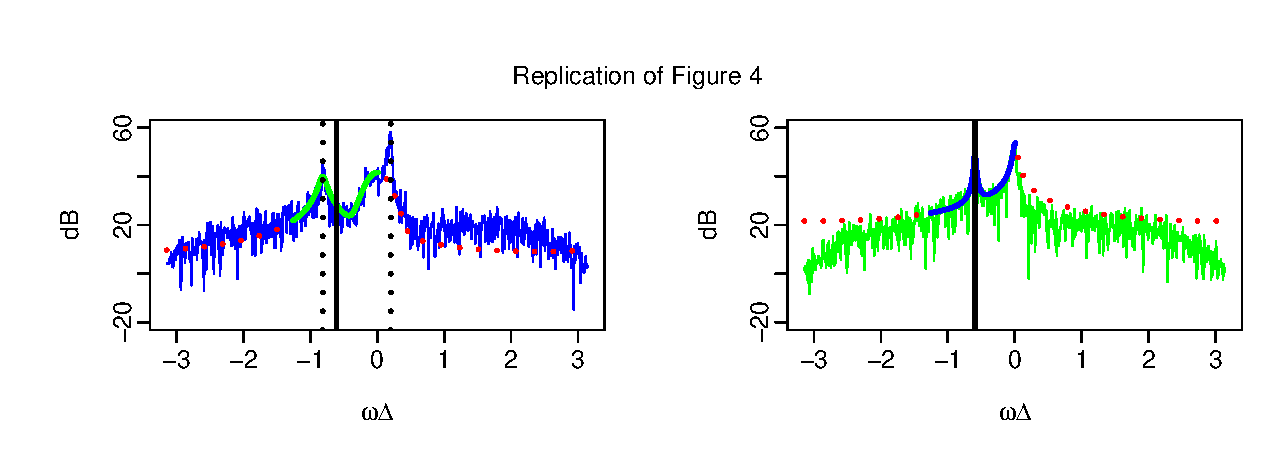
\includegraphics[width=\textwidth]{ReplicatedFigures/fig4.pdf}
        \caption{Periodograms of the time series sections colored blue and green in Figure \ref{fig: fig1}. The black line denotes the inertial frequency.   The dotted lines on the left figure indicate the location of the eddy peak and the expected shift in the inertial frequency. The semi-parametric model fit for the frequencies used in model fitting is highlighted green on the left figure and blue on the right figure. The red dotted line indicates the model fit extended beyond the frequencies where it was fit. }
        	\label{fig: fig4}
\end{figure}


\subsubsection{Non-stationarity}
To allow for non-stationarity in long time series, \citet{Sykulski2016} propose fitting the model independently at each observed time point using a rolling window around the time point of interest. 
This makes parameters in the OU differential equation
\begin{equation}
dz(t) = \{i \omega_{0}(t) - c(t) \} z(t) dt + A(t) dQ(t)
\end{equation}
and power spectral density
\begin{equation}
S^{(0)}(\omega, t) = \frac{A(t)^{2}}{(\omega - \omega_{0}(t))^{2} + c(t)^{2}}
\end{equation}
 now be a functions of time. 
Similarly, the time-varying version of the Mat\'{e}rn power spectral density is 
\begin{equation}
S^{(m)}(\omega, t) = \frac{B^{2}(t)}{(\omega^{2} + h^{2}(t))^{\alpha(t)}}.
\end{equation}
The length of the window to fit these time-varying parameters needs to be large enough to provide good estimation of the spectrum, but short enough to be treated as locally stationary. 
 In this analysis, the authors select a reasonable window length empirically, but acknowledge that further work on this subject would be of value.  

\subsubsection{Significance tests for simpler models}
\label{sec: sig}
Finally, \citet{Sykulski2016} propose that a simple likelihood ratio test can be used at each time period to test whether or not a shift in the inertial oscillation has occurred. 
To do so, the authors suggest fitting a simpler five parameter model where the the parameter $\omega_{0}$ is fixed to be the inertial frequency $f_{0}$. 
Then this simpler model can be compared to the full six parameter model via a likelihood ratio test with test statistic
\begin{equation}
\label{eq: LRT}
R(t) = 2[l_{b} \{\hat{\theta}_{1}(t) \} - l_{b}\{\hat{\theta}_{0}(t) \} ],
\end{equation}
where $\hat{\theta}_{0}(t)$ is the fitted parameter vector for the simpler, or null model, and $\hat{\theta}_{1}(t)$ is the fitted parameter vector for the full model.
 The authors claim $R(t)$ then follows a chi-squared distribution with 1 degree of freedom. 
 However, as we will discuss further, this may be overly simplistic, because of potential identifiability issues with the parameters and lack of independence between time points stemming from the use of a rolling window. 
 

\section{Results}
\subsection{Simulated data}
\par We show the potential utility of this method by analyzing two non-trivial data sets.  
First, we consider the modeled trajectories of 200 near-surface particles obtained from a computer simulation of ocean circulation, where each of the trajectories are recorded at two hour intervals. 
The simulation is set to be `very similar' to the SPEM 5.2 set-up of \citet{Danioux2008}. 
In the  simulation, the turbulence is designed to be at a steady-state and wind forcing is set to be  constant. 
The simulated data is useful as a verification tool, since  it contains no eddies and its only  notable asymmetry between the two directions of rotation is due to the inertial oscillations. 


\par For all two hundred trajectories, the full six-parameter model, given in Equation \ref{eq: fullSpec}, is fit to each trajectory. 
The model is fit using both sides of the spectrum with frequencies up to 1.5 times the inertial frequency. 
The parameters are assumed constant, since this portion of the time series does is fairly short. 
In Figure \ref{fig: fig5}, we display the fit of the aggregate spectral model to a single trajectory from the simulation and to an ensemble of trajectories. 
We also display the individual periodograms and model fits. 
The resulting spectra consistently have peaks at zero and at the inertial frequency, which indicates that the model captures the turbulent background and the inertial oscillations accurately. 
\citet{Sykulski2016}  note that this highlights the method's robustness, since the individual periodograms show considerable variability, but the model fits are all quite consistent.

\begin{figure}[h!]
  \centering
    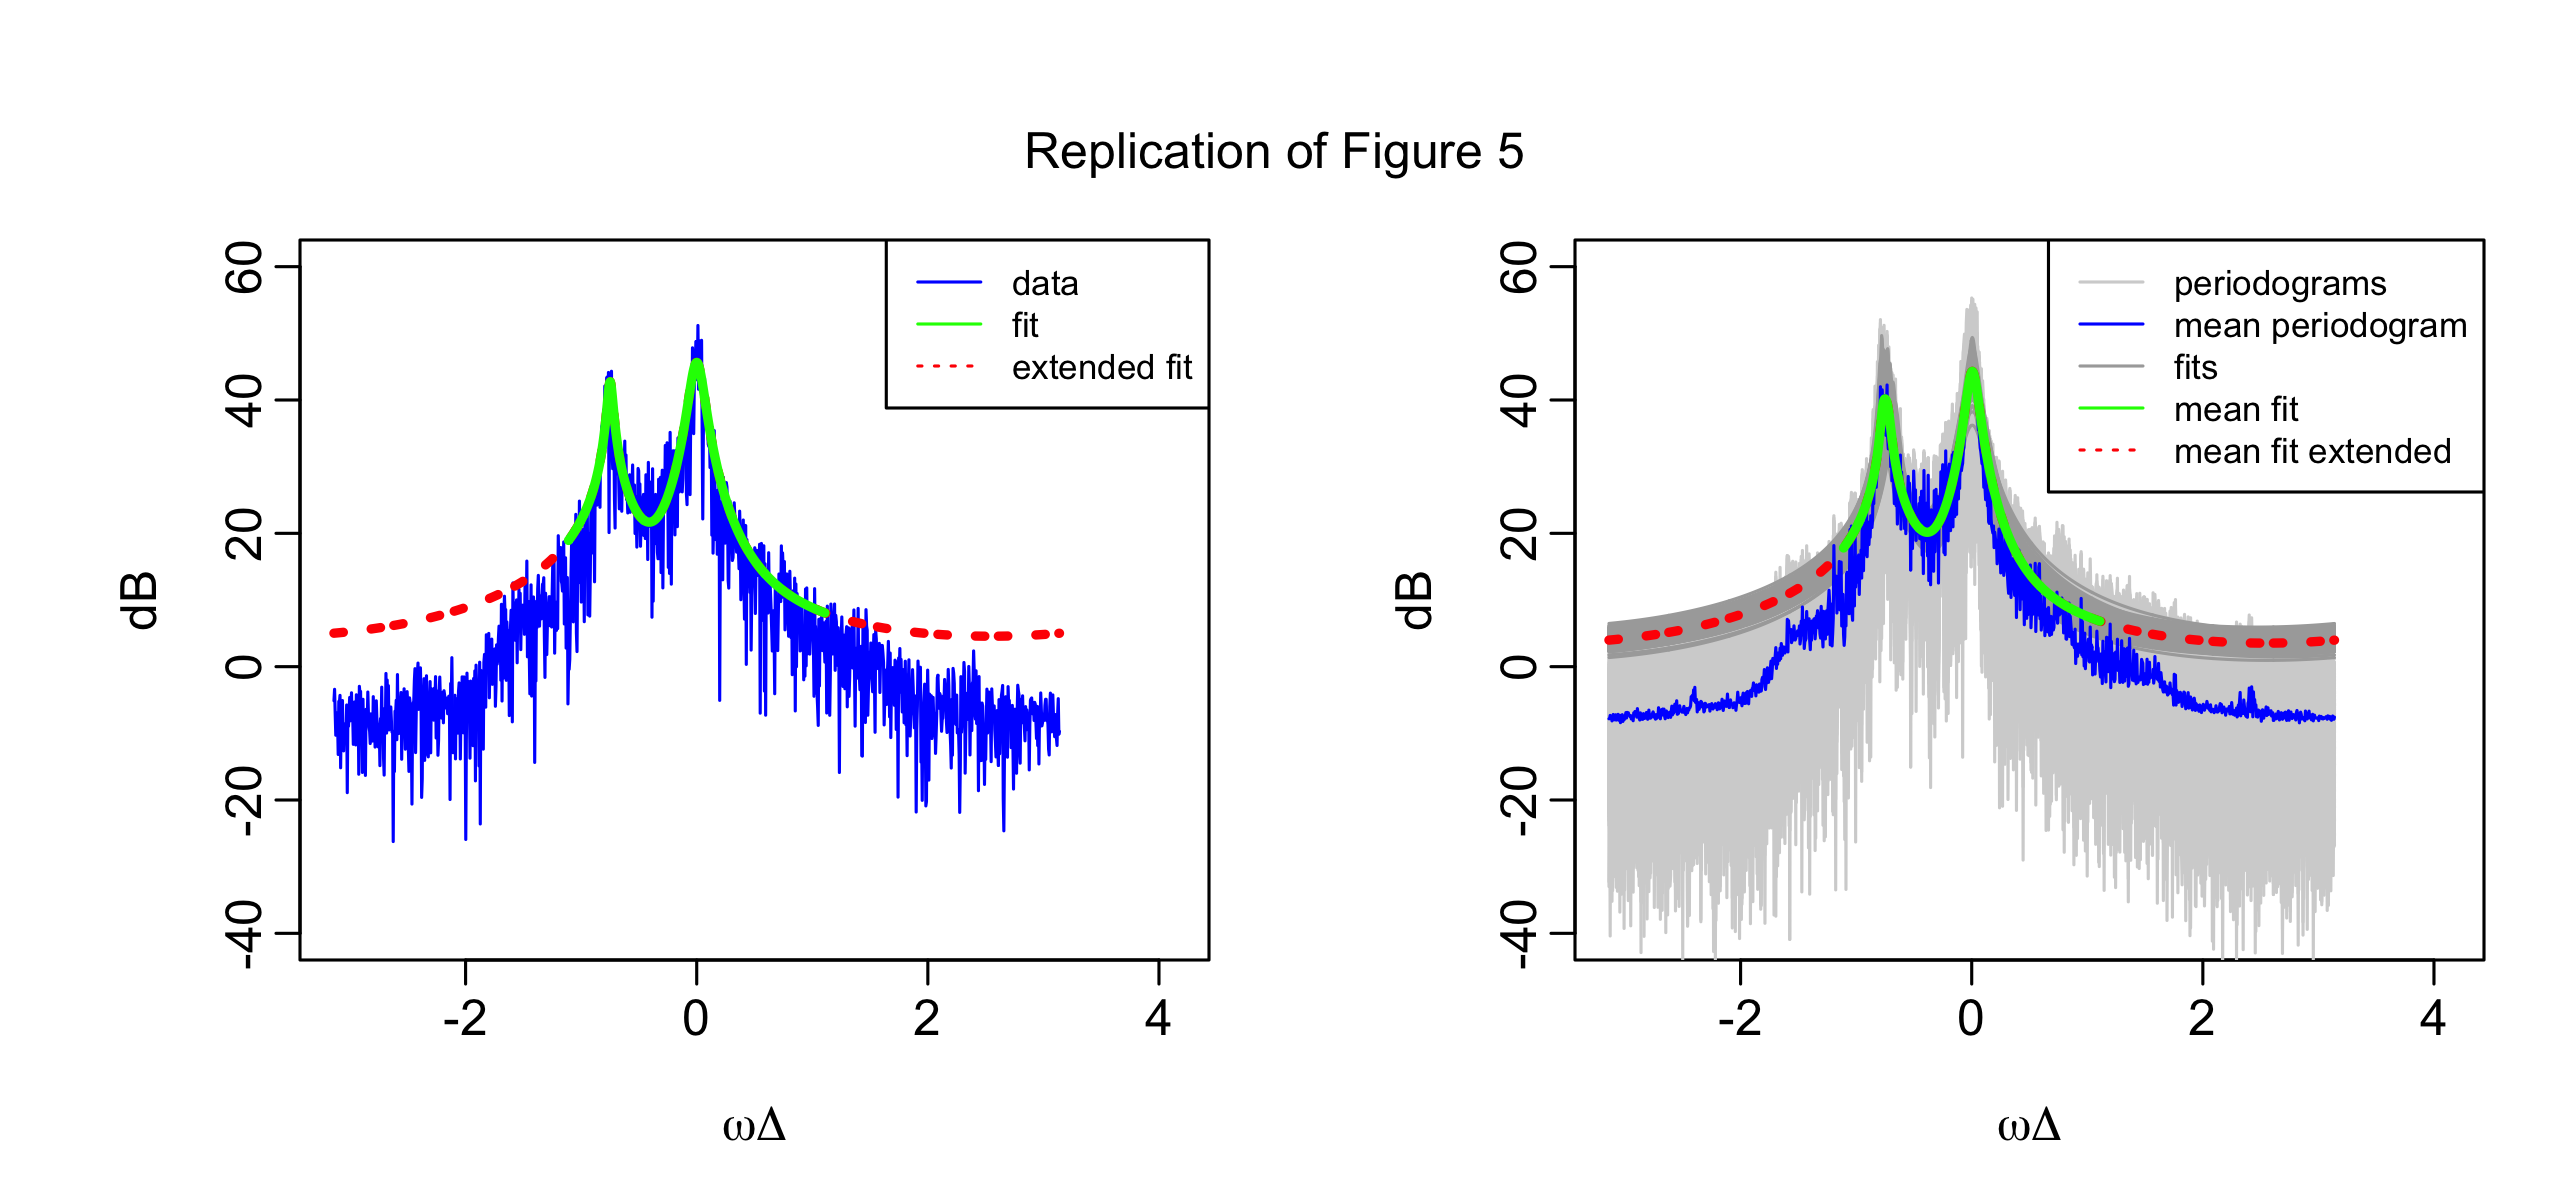
\includegraphics[width=\textwidth]{ReplicatedFigures/fig5.png}
        \caption{Left: The spectral density of one particle (blue) with the model fit overlaid for the portion of the spectra used to fit it (green) and extended to all frequencies (red). Right: The ensemble mean periodogram (blue) with the ensemble fit for the frequencies used to fit it (green) and extended to the entire spectrum (red). Individual trajectories' periodograms (light grey) and model fits (dark fit) are also displayed. }
        \label{fig: fig5}
\end{figure}

\subsection{South Pacific Drifter}
\label{sec: spDrift}
We also consider the trajectory of a drifter in the south Pacific ocean observed 12 times a day over a 1642 day period.  
The trajectory is displayed in the left panel of Figure \ref{fig: fig6}. 
We first consider fitting a 20-day sample of this trajectory. 
Its periodogram, displayed in Figure \ref{fig: fig6}, shows substantial asymmetry between the positive and negative frequencies. Thus, the semi-parametric approach is applied and only positive frequencies are used in fitting the model. 

\begin{figure}[h!]
  \centering
    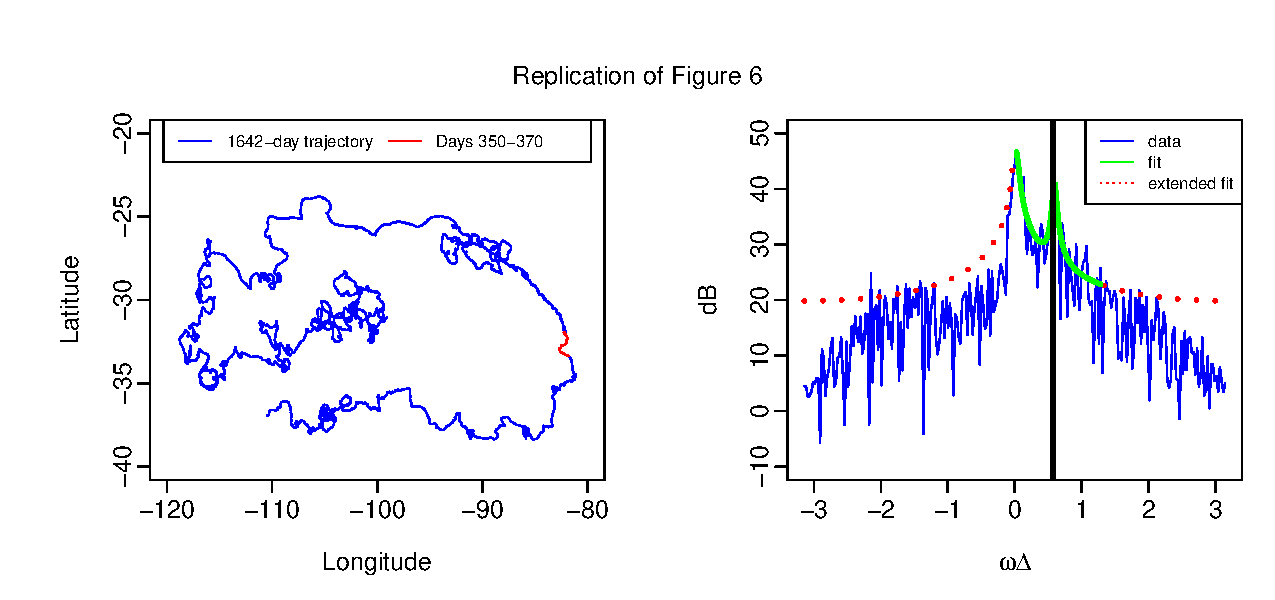
\includegraphics[width=\textwidth]{ReplicatedFigures/fig6.pdf}
        \caption{Left: The trajectory of the drifter in the south Pacific ocean. Right: The periodogram and model fit for the section of the trajectory highlighted in red. The green portion of the model fit corresponds to the frequencies used in fitting and the red dotted line is an extension of the fit to other frequencies. }
        \label{fig: fig6}
\end{figure}

\par
Moving on to the entire time series, we use rolling windows of 1000 observations and the semi-parametric set-up described in Section \ref{sec: semi}  to obtain parameter estimates for the spectral model at each time point.
 In Figure \ref{fig:timeVarying}, we compare the observed spectral density over time and the fitted spectral density in a time-frequency plot. 
  The fitted density appears to be a smoothed version of the observed density,  indicating a reasonable model fit.
   Typically the inertial frequency matches the Coriolis frequency, which would be expected given that shifts from the Coriolis frequency are only rare events.
   
   \begin{figure}[h!]
  \centering
    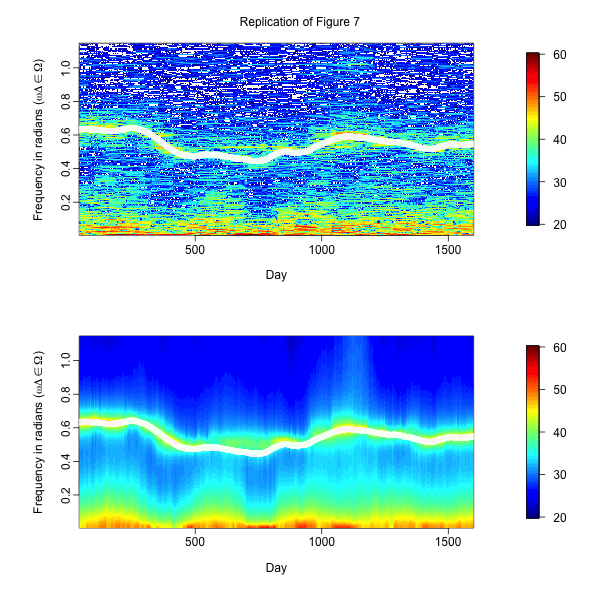
\includegraphics[width=\textwidth]{ReplicatedFigures/fig7.png}
        \caption{Top: Observed spectra of the drifter over time; Bottom: Modeled spectra over time. On both figures, the semi-transparent gray line indicates the average inertial frequency within the rolling window at the current time period.  Only frequencies used in the estimation are included.  }
        	\label{fig:timeVarying}
\end{figure}

   
 \par
 We also display the fitted parameter values over time and their 95$\%$ confidence interval bands in Figure \ref{fig: fig8}. 
The 95$\%$ intervals are obtained using numerical calculation of the Hessian.
The parameters all change smoothly over time. 
We note that the inertial frequency differs from the Coriolis Frequency from roughly days 600 to 900. 
\citet{Sykulski2016} note that this deviation is appropriate and can be explained by a change in tidal energy over shallow periods of water. 
 \begin{figure}[h!]
  \centering
    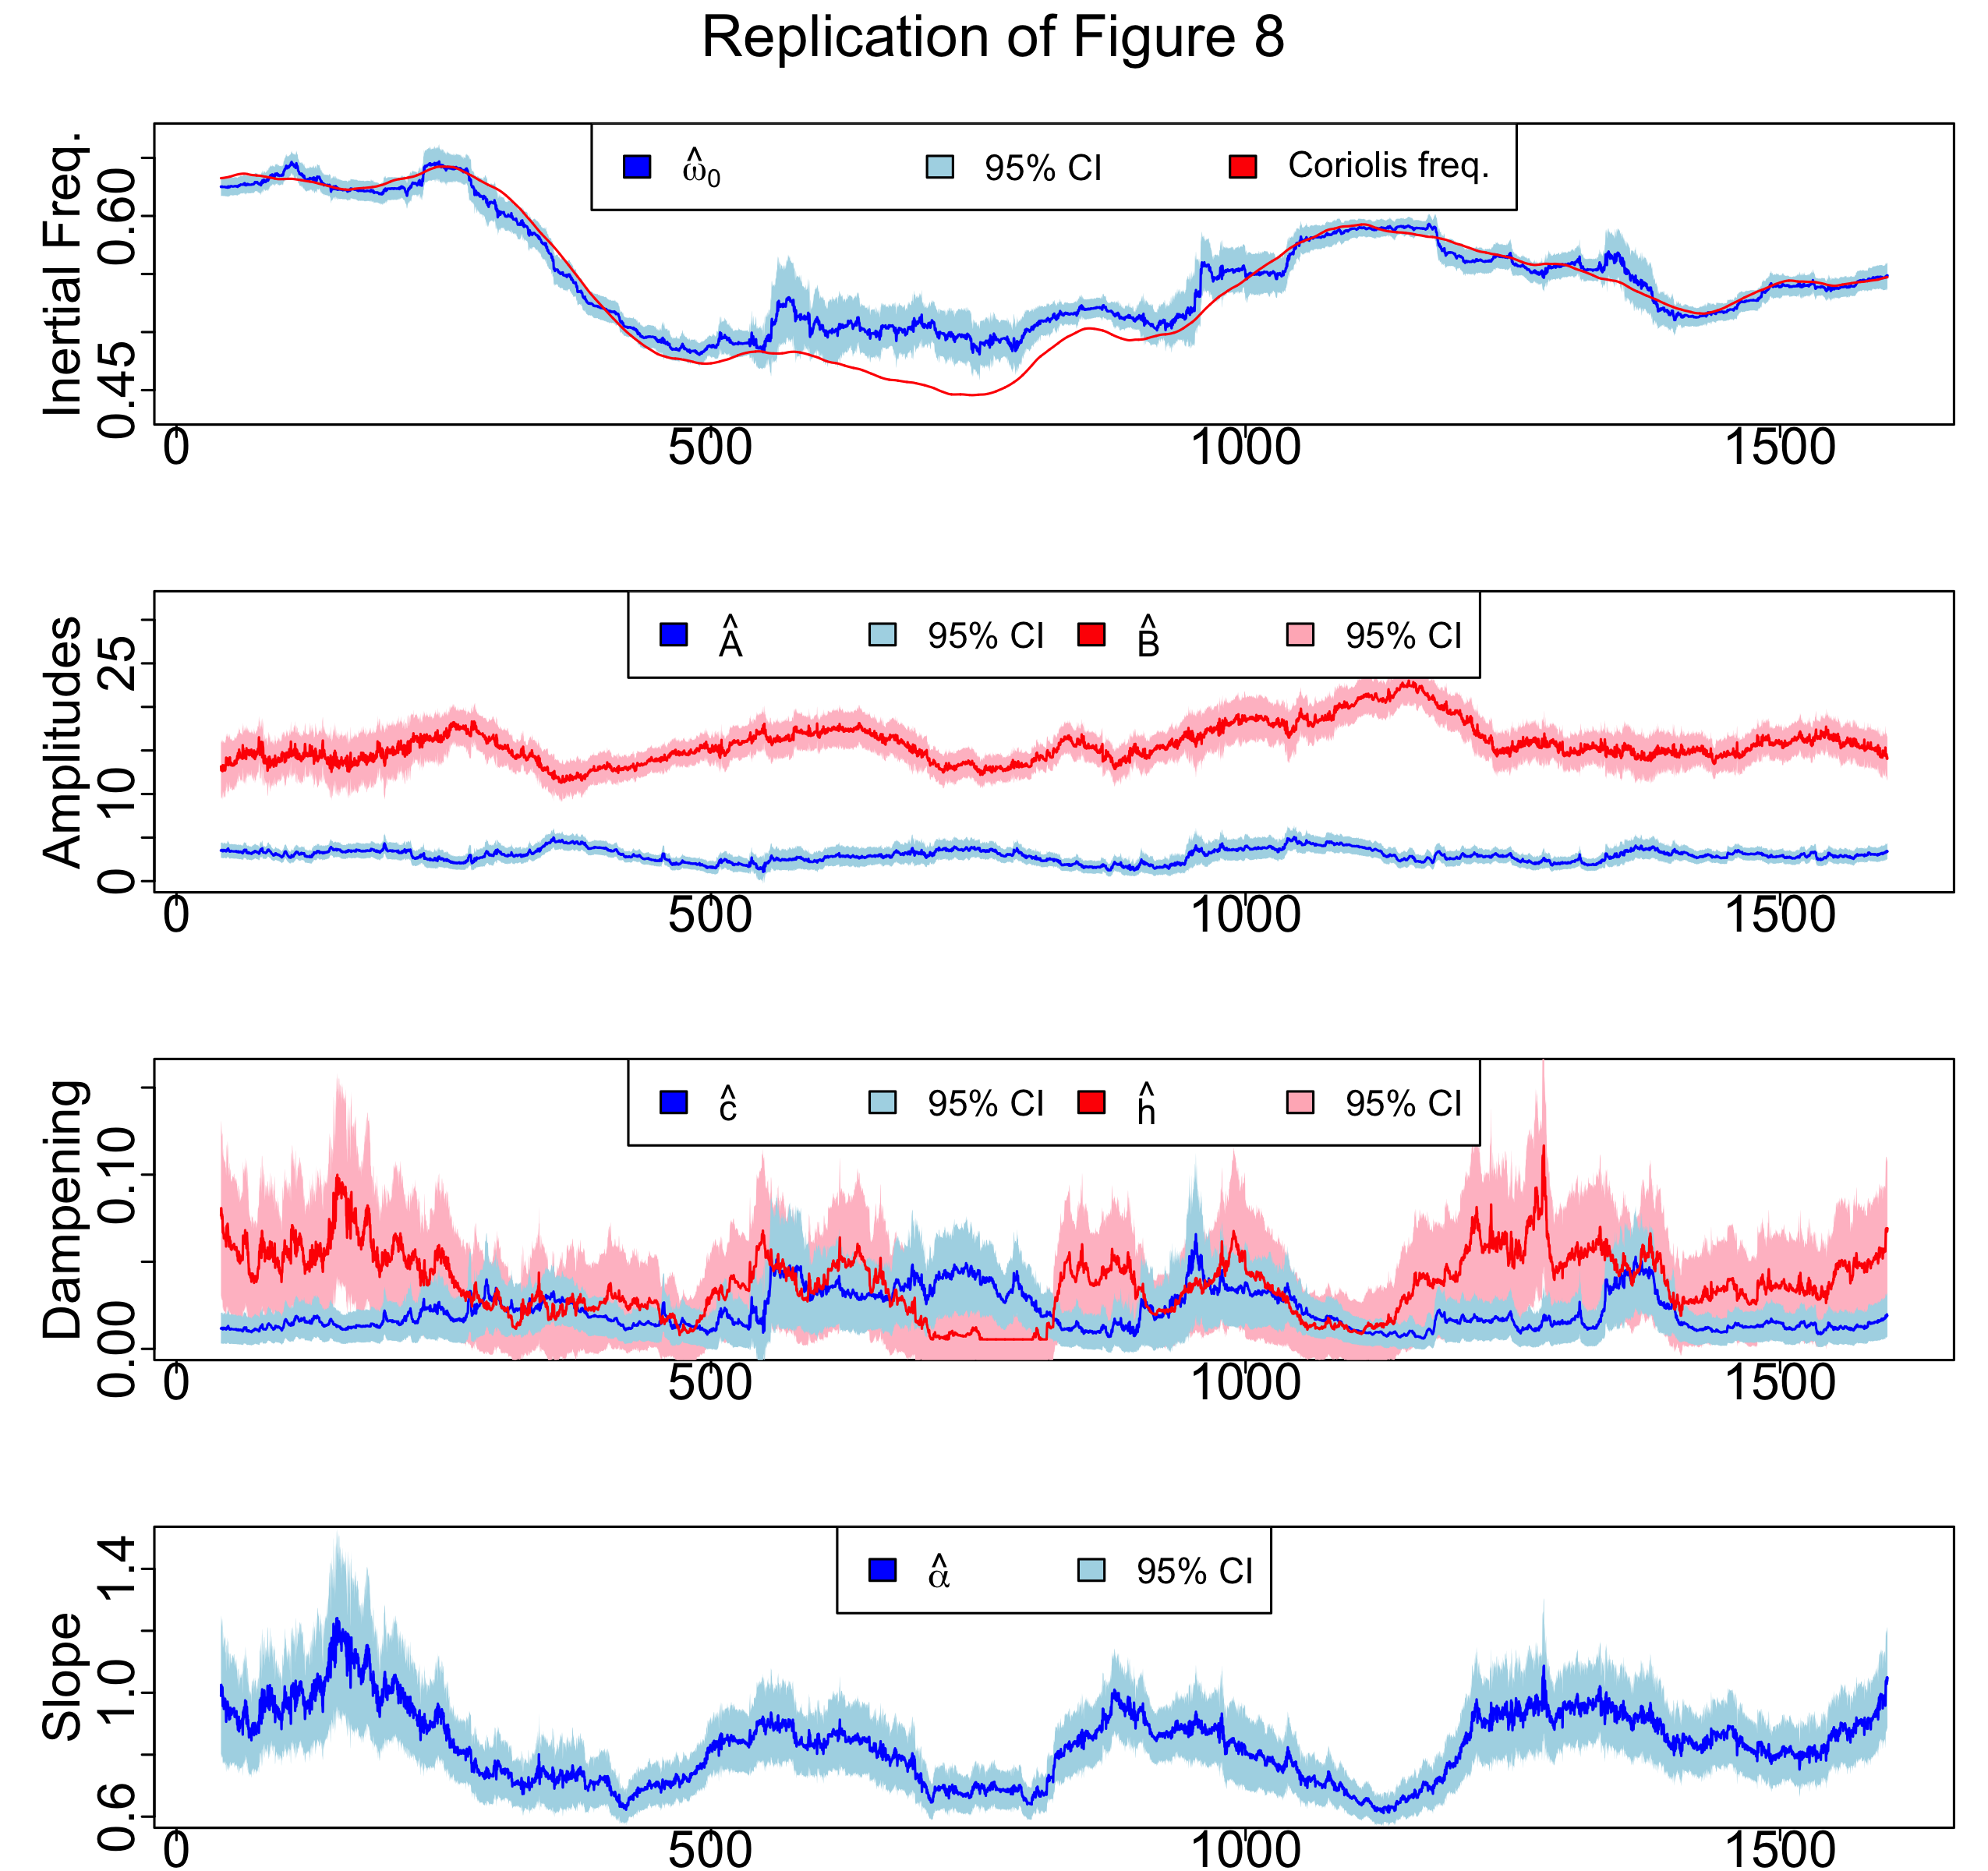
\includegraphics[width=\textwidth]{ReplicatedFigures/fig8.png}
        \caption{Estimates of the six model parameters overtime with 95$\%$ confidence interval bands. The red line in the top figure is the inertial frequency.}
        	\label{fig: fig8}
\end{figure}

 \begin{figure}[h!]
  \centering
    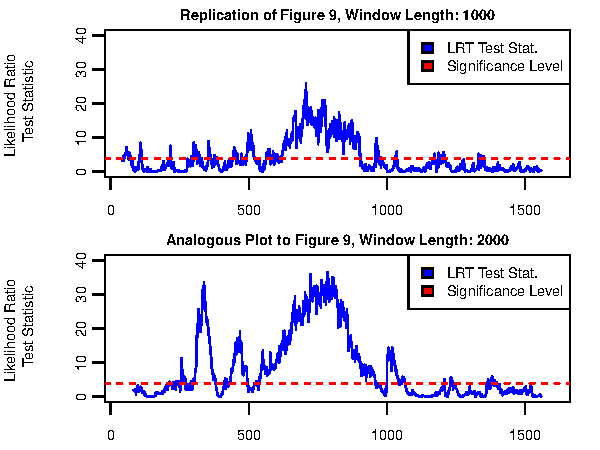
\includegraphics[width=.85\textwidth]{ReplicatedFigures/fig9Extend.pdf}
        \caption{Time series of the likelihood ratio test statistic comparing the 5-parameter to 6-parameter models. The dotted red line indicates the value at which test statistics indicate a significant difference between the model. The first figure uses the window size specified in \citet{Sykulski2016} and the second figure doubles the window size.}
        	\label{fig: fig9}
\end{figure}

   
   

\par We also fit the 5-parameter model where the frequency is set to the inertial frequency rather than being a free-parameter. 
We then compare this fit to the full model using a likelihood ratio test as described in Section \ref{sec: sig}.
 In Figure \ref{fig: fig9}, we display the test statistics over time where a red line is used to indicate the level of statistical significance. 
The authors conclude that when there are statistically significant differences between the 5-parameter and 6-parameter model, as indicated by the likelihood ratio test,   the inertial frequency does not equal the Coriolis frequency.   
They note that the period from days 600 to 900 always shows a significant difference between the models, which corresponds to the period of shifts observed in Figure \ref{fig: fig8}.

\par We, however, are skeptical of this use of simple hypothesis testing. 
The parameters are being estimated repeatedly using a rolling window. 
This means that there is not independence between the time periods and there is repeated testing. 
Both of these issues should be accounted for in designing a hypothesis test. 
Further, the authors acknowledge elsewhere in the paper that the length of the rolling window is currently selected empirically and that further work on selecting windows would be beneficial. 
This suggests that the p-value for any time point could be easily influenced by the length of the window used in fitting it.
To explore this, in Figure \ref{fig: fig9} we replicate Figure 9  in the paper using both the window length specified in the paper and a doubled window length.
The corresponding likelihood ratio tests do not reject the null hypothesis at all the same times. 
This indicates that window size and its influence on hypothesis testing should be further investigated prior to applying this formal testing approach for the presence of a shift from the Coriolis frequency. 




 \begin{figure}[h!]
  \centering
    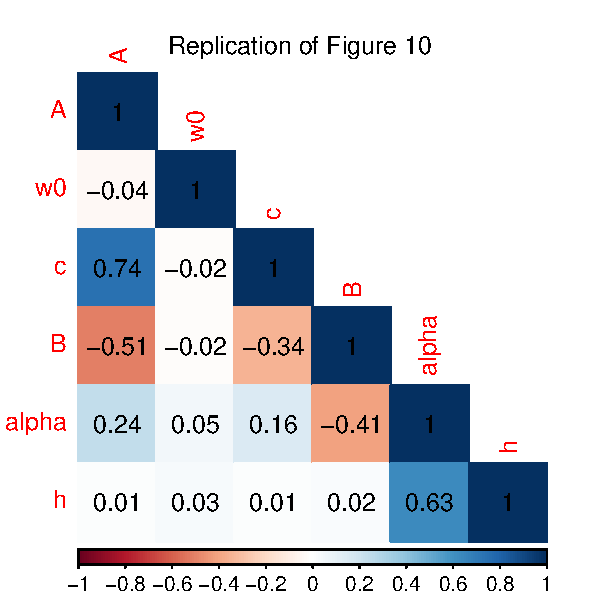
\includegraphics[width=.6\textwidth]{ReplicatedFigures/fig10.pdf}
        \caption{Table of the average correlation between parameters. Note that there are  minor differences in the correlation values between these results and those in \citet{Sykulski2016} These differences can be attributed to slight differences in the numerical optimization used by R and Matlab in calculating the Hessian. }
        	\label{fig: fig10}
\end{figure}


\par Finally, in Figure \ref{fig: fig10}, we display a matrix of the average correlation of the parameters over time. \citet{Sykulski2016} highlight several useful results from this table. 
They note that the inertial frequency is generally uncorrelated with other parameters values, suggesting that the inertial frequency only controls the location of the peak, but does not influence the shape or amplitude of the spectra as desired. 
They also highlight the many correlations between parameters that are part of the turbulent background component and inertial oscillation components of the model. 
This indicates that these two aspects of the ocean's behavior are linked and should be modeled together as has been done in this paper. 




\section{Discussion}
\par Overall, \citet{Sykulski2016} present a  well-developed model for capturing the behavior of ocean surface drifters.
 In particular, they develop a two component spectral model that jointly accounts for the turbulent background behavior of the ocean and the influence of inertial oscillations. 
 Using the complex-valued OU process, the authors develop a stochastic analogue to the accepted deterministic differential equations used to describe this phenomena. 
 In so doing, they are the first to explicitly model inertial oscillations within the context of a stochastic model. 
 Further, to model the turbulent background, the authors propose using the  Mat\'{e}rn autocovariance structure.
  This flexible model cleverly encompasses all models that have previously been proposed for the turbulent background as special cases.
  This allows the data to determine what is the most appropriate behavior. 
   They also employ the newly-developed Blurred Whittle likelihood for model fitting, which compensates for bias and aliasing, unlike typical Whittle likelihood. 
   All together, this spectral model provides an automated way to detect shifts from the Coriolis frequency in a long time series. 
This provide an efficient way to detect eddies for large numbers and/or long time series. 
So, the authors have  satisfied their scientific, and, in so doing, introduced new statistical ideas.

Nevertheless, despite its overall sophistication, some areas in the paper could be improved. 
As discussed in Section \ref{sec: spDrift}, the simple likelihood ratio test proposed in the paper may not be sufficient for the involved, time-varying model used in the paper.  
Another area that is insufficiently addressed in the paper is possible identifiability issues between the model parameters. 
 If parameter estimates are highly correlated, physical changes in one parameter might actually be reflected by changes in other fitted parameters.
  This would subsequently invalidate conclusions about observed changes in specific parameters, since they could be masked by changes in other parameters. 
 For example, in Figure \ref{fig: fig10}, we see a high correlation (0.74) between the OU dampening and amplitude parameters, suggesting caution should be taken in interpreting their physical meaning. 
 For the primary variable of interest, inertial frequency, all correlations with other parameters are low, so the main conclusions of the paper are not affected by this issue. 
Nevertheless, a fuller discussion of these limitations in interpretation would have been valuable.
\par Overall, \citet{Sykulski2016} present a novel method for modeling ocean surface drifters.
 Their work is a substantial contribution to stochastic modeling, particularly, in terms, of explicitly incorporating known physics into statistical models. 




\clearpage

\bibliography{prelim}


\section{Appendix}

\subsection{Errata}
We note a few minor errors in the paper.
\begin{itemize}
\item Equation 13 has a typo. The second term in the sum should exactly match Equation 6. 
\item In Figure 6, the periodogram and model fit are for days 350 to 370 not days 358 to 378. (This is apparent from looking at the author's code.)
\item In Figure 10, the fifth row in the table should be labeled $\alpha$ and not $\delta$.
\end{itemize} 

\subsection{Additional Replicated Figures}

\begin{figure}[h!]
  \centering
    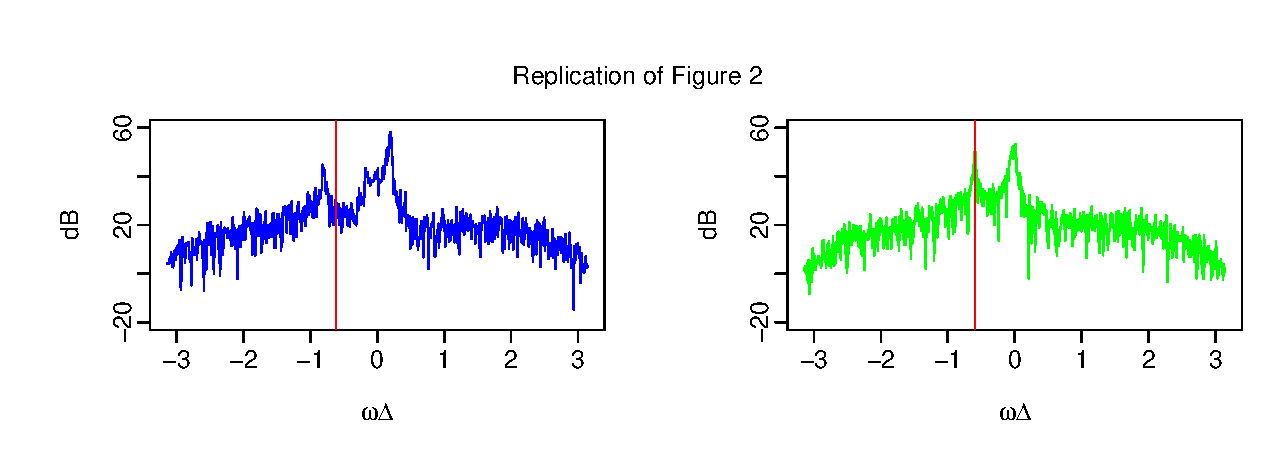
\includegraphics[width=\textwidth]{ReplicatedFigures/fig2.pdf}
        \caption{Periodograms of the highlighted green and blue sections of the trajectories in Figure \ref{fig: fig1}. The inertial frequencies are marked in red. }
        	\label{fig: fig2}
\end{figure}




\end{document}

